\chapter{Fundamentos de eletromagnetismo}\label{sec.fund_eletr}

\section{Introdução}

\section{Fatos experimentais}
De acordo com \cite{jackson_classical_1999} e \cite{sommerfeld_52} , os conceitos, definições e resultados em eletromagnetismo clássico partem das experiências de Cavendish e Coulomb no final do Séc. $XVIII$. A partir desses experimentos foi estabelecida a Lei de Coulomb
\begin{equation}\label{eq.forc_elet}
\textbf{F}=k\,\frac{q_1\,q_2}{||\textbf{x}_1-\textbf{x}_2||^2}\frac{\textbf{x}_1-\textbf{x}_2}{||\textbf{x}_1-\textbf{x}_2||},
\end{equation}
onde $q_i$ são as cargas elétricas (campos escalares) presentes nos pontos $\textbf{x}_i$, respectivamente, $k$ (campo escalar) é uma constante de proporcionalidade cujo valor depende do sistema de unidades de medida adotado, $||\textbf{x}_1-\textbf{x}_2||^2$ é a distância euclidiana entre as cargas e $\textbf{F}$ é a força elétrica exercida pela carga $q_2$ sobre a carga $q_1$. As notações em negrito representam campos vetorias pertencentes ao espaço $\mathbb{R}^3$, e o vetor normal que fornece a direção de interação entre as cargas é dado por $(\textbf{x}_1-\textbf{x}_2)/||\textbf{x}_1-\textbf{x}_2||$.

O campo elétrico $\textbf{E}$ foi definido como sendo a força elétrica por unidade de carga em um determinado ponto, portanto é uma função vetorial que depende de sua posição em relação à carga, ou seja,
\begin{equation}\label{eq.camp_elet}
\textbf{F}=q\,\textbf{E}.
\end{equation}
Experimentalmente, tanto a direção da força como a razão entre a força e a quantidade de carga vão se tornando constantes à medida que a quantidade de carga se torna cada vez menor, definindo a magnitude e a direção do campo elétrico. No SI, a unidade de medida de carga é o \textit{coulomb} $(C)$, o campo elétrico é o \textit{newton/coulomb} $(N/C)$ ou o \textit{volt/metro} $(V/m)$, e a constante $k=(4\pi\,\epsilon_0)^{-1}$ onde $\epsilon_0\simeq8.854\times10^{-12}$ é a permissividade elétrica no vácuo medida em \textit{farad/m} $(F/m)$.

Substituindo a equação \ref{eq.camp_elet} em \ref{eq.forc_elet} temos que o campo elétrico agindo num ponto $\textbf{x}$ qualquer devido a uma carga $q_1$ no ponto $\textbf{x}_1$ é
\begin{equation*}
\textbf{E}=k\,\frac{q_1}{||\textbf{x}_1-\textbf{x}_2||^2}\frac{\textbf{x}_1-\textbf{x}_2}{||\textbf{x}_1-\textbf{x}_2||},
\end{equation*}
como podemos observar na figura tal simulando um sistema de coordenadas qualquer.
\begin{figure}
\centering
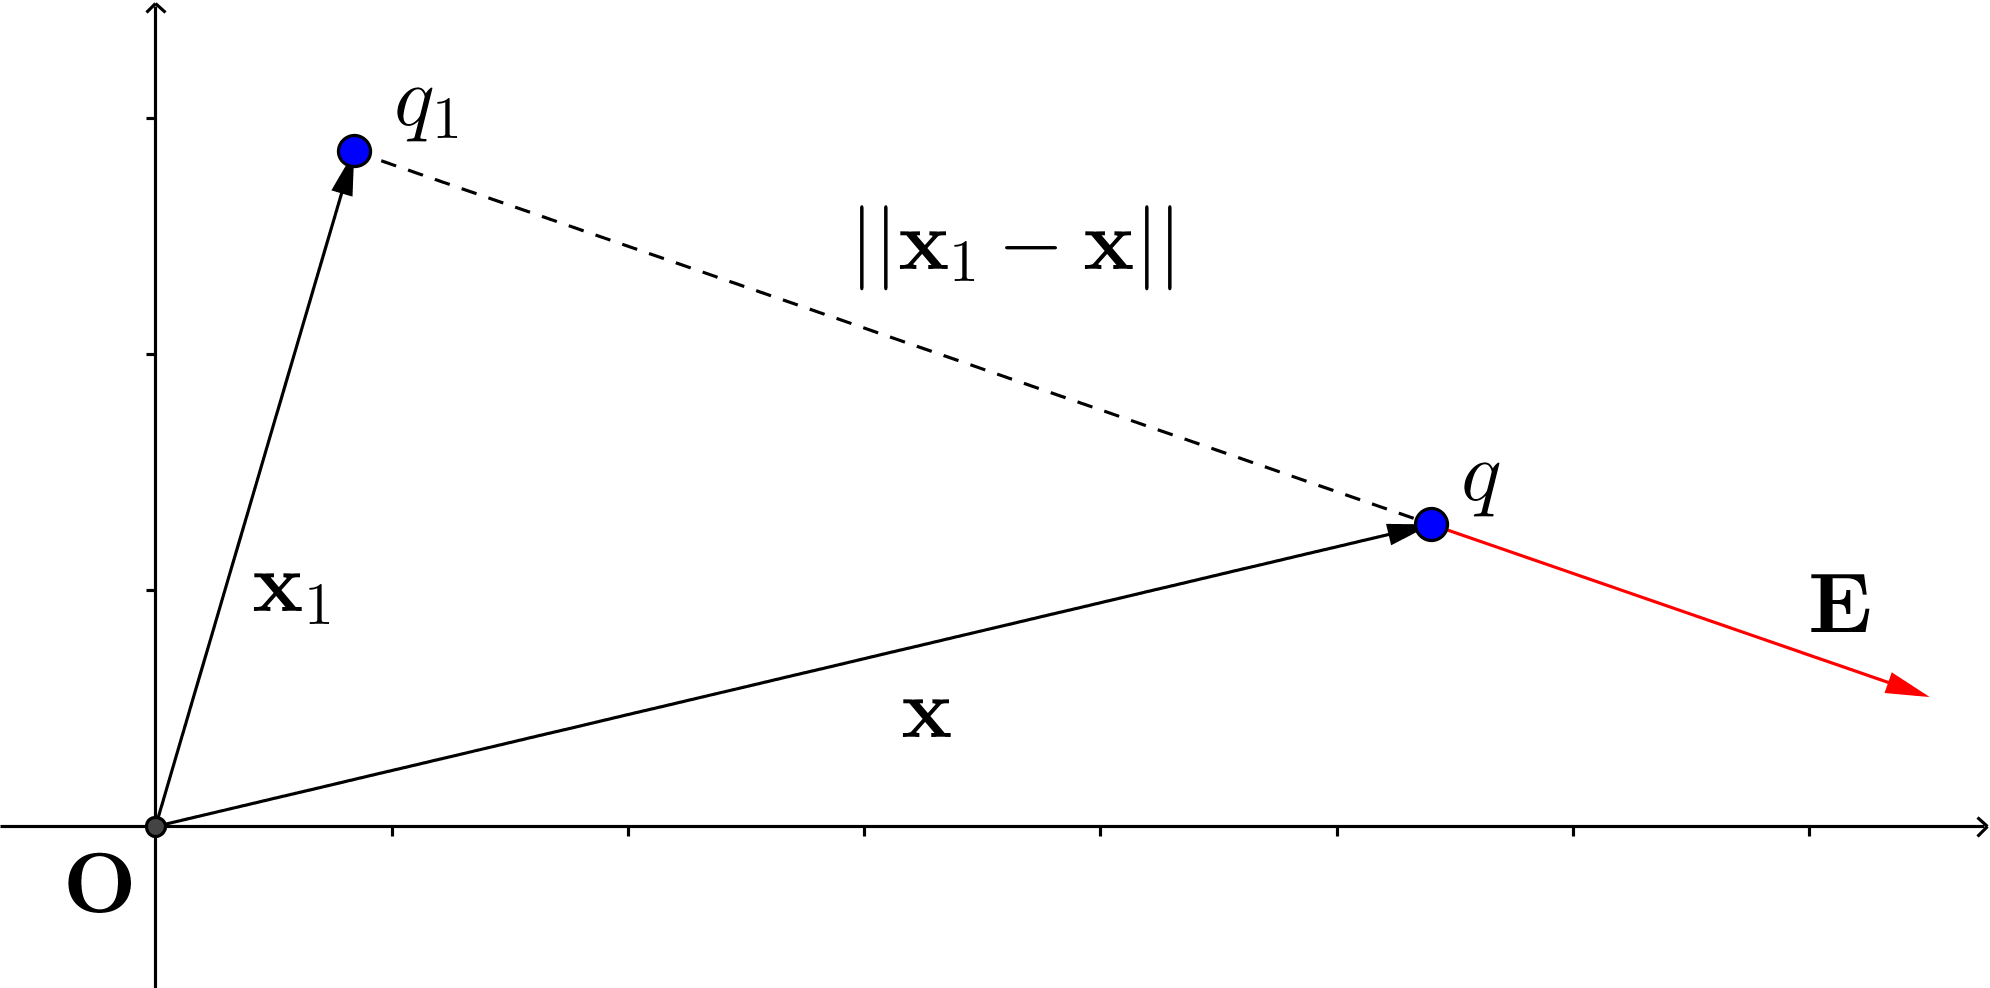
\includegraphics[scale=1.5]{camp_elet}
\caption{\textit{Exemplificação da interação entre cargas elétricas devido à geração, em função de $q_1$, de um campo elétrico. A força elétrica $\textbf{F}$ atuando numa carga qualquer $q$ tem mesma direção do campo elétrico $\textbf{E}$, com mesmo sentido ou sentido oposto conforme a carga $q_1$ é positiva ou negativa, respectivamente.}}
\label{fig.camp_eletr}
\end{figure}

\begin{figure}[!htb]
\centering
\subfloat{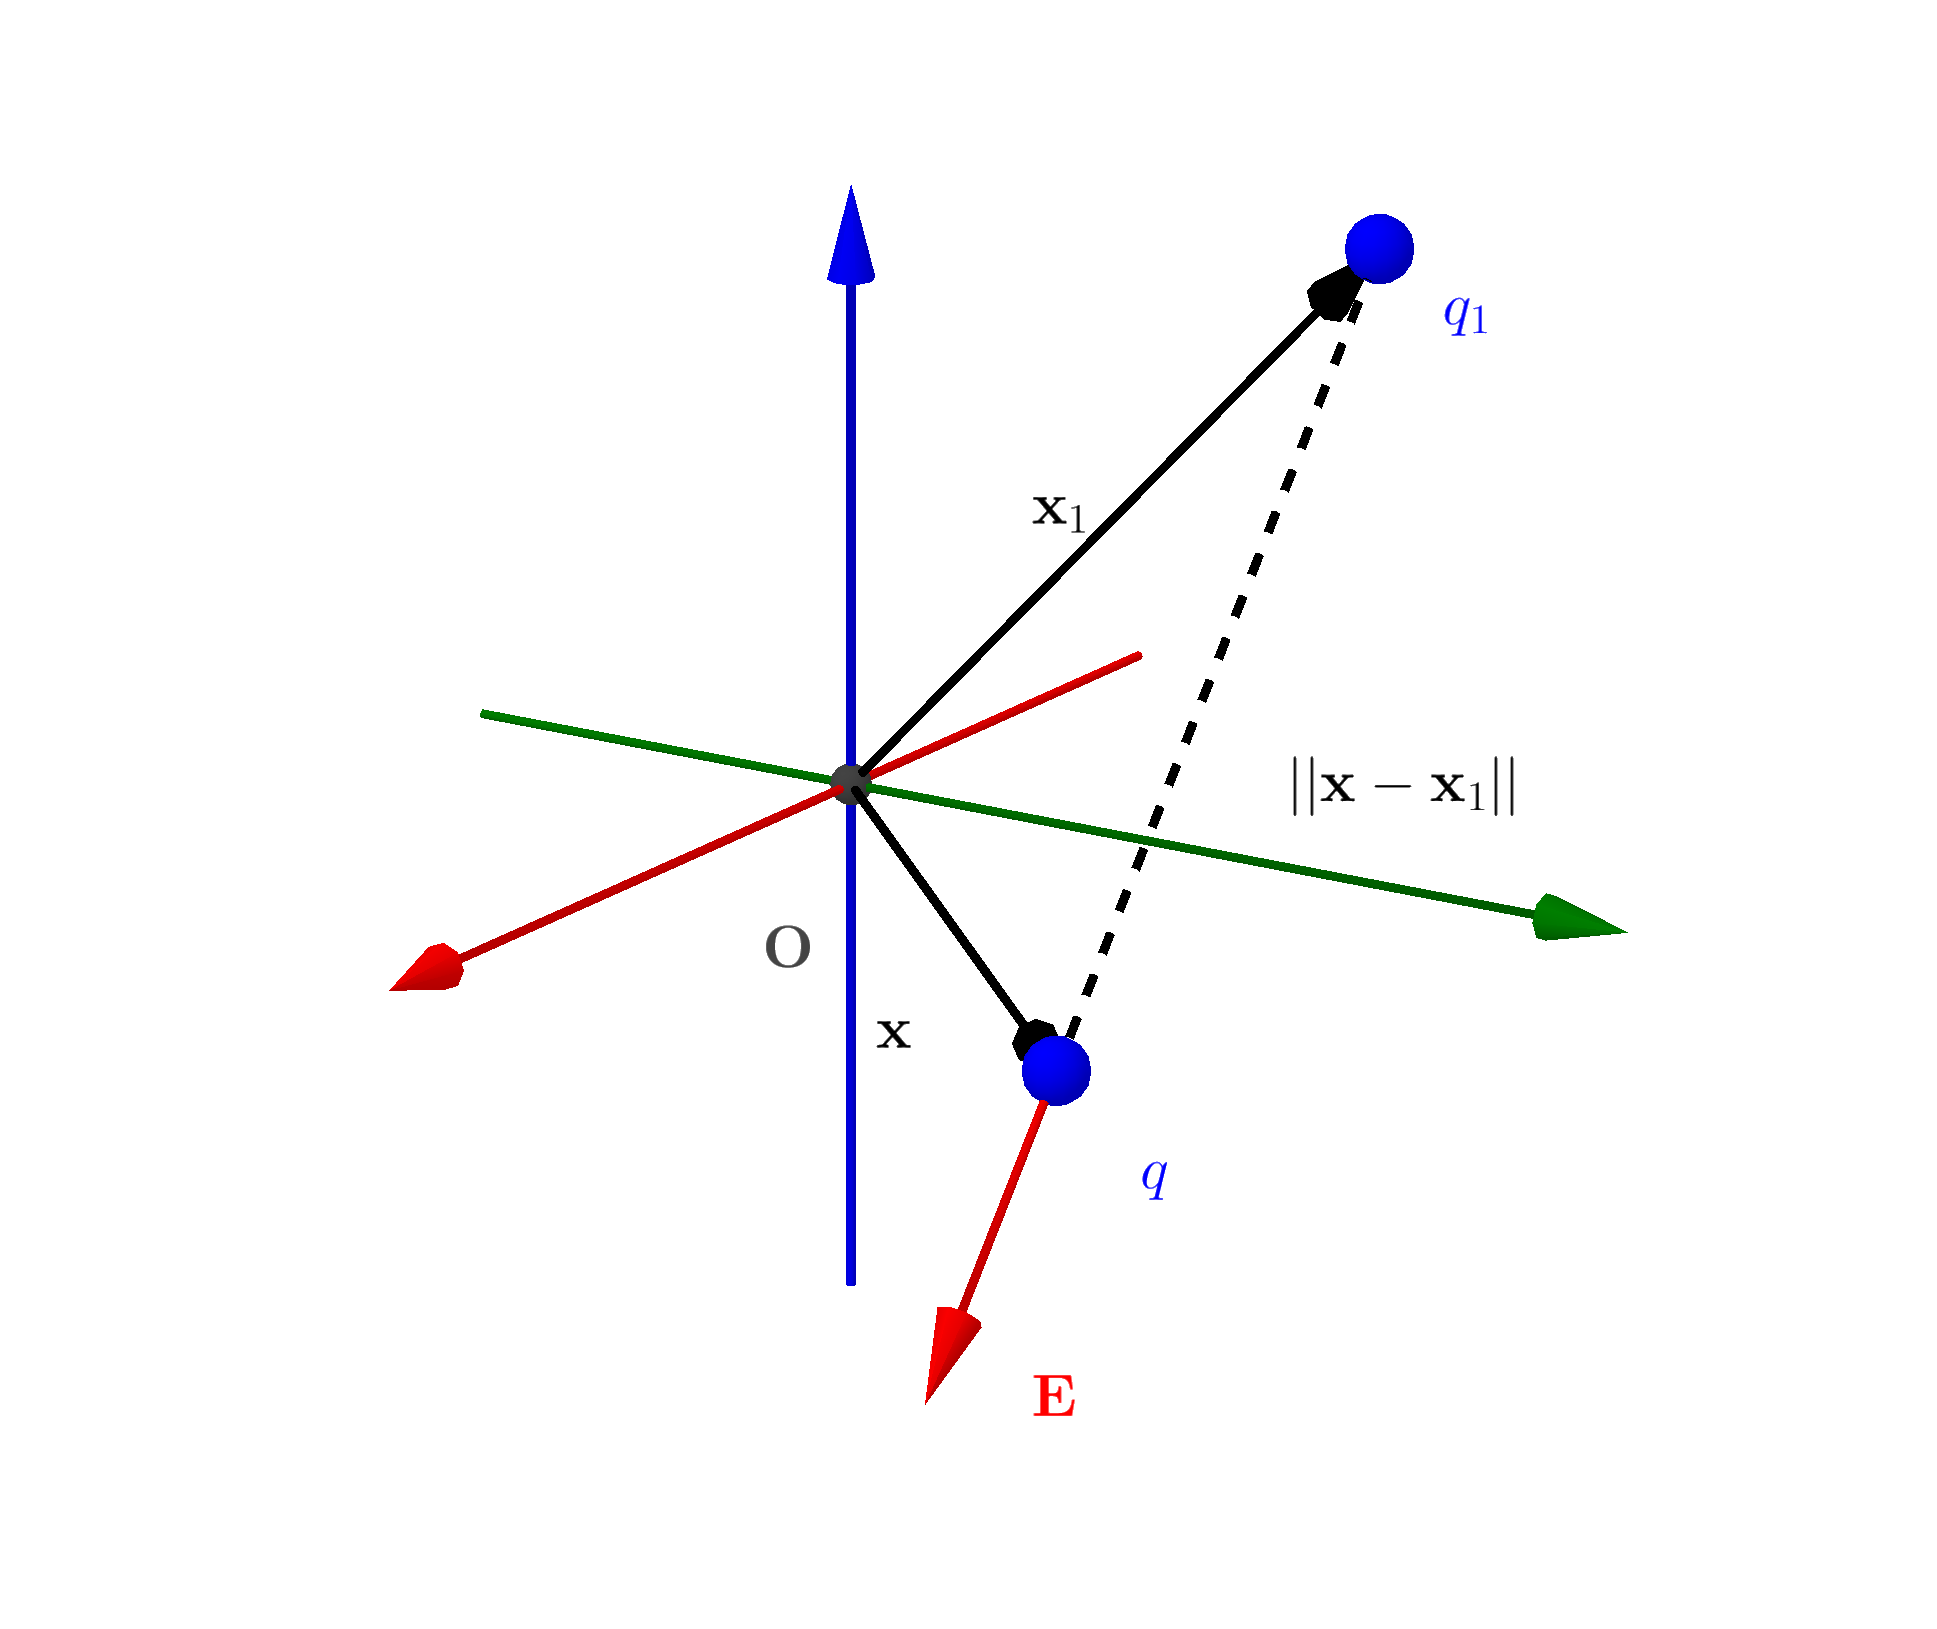
\includegraphics[scale=1]{camp_elet_3D}}
\subfloat{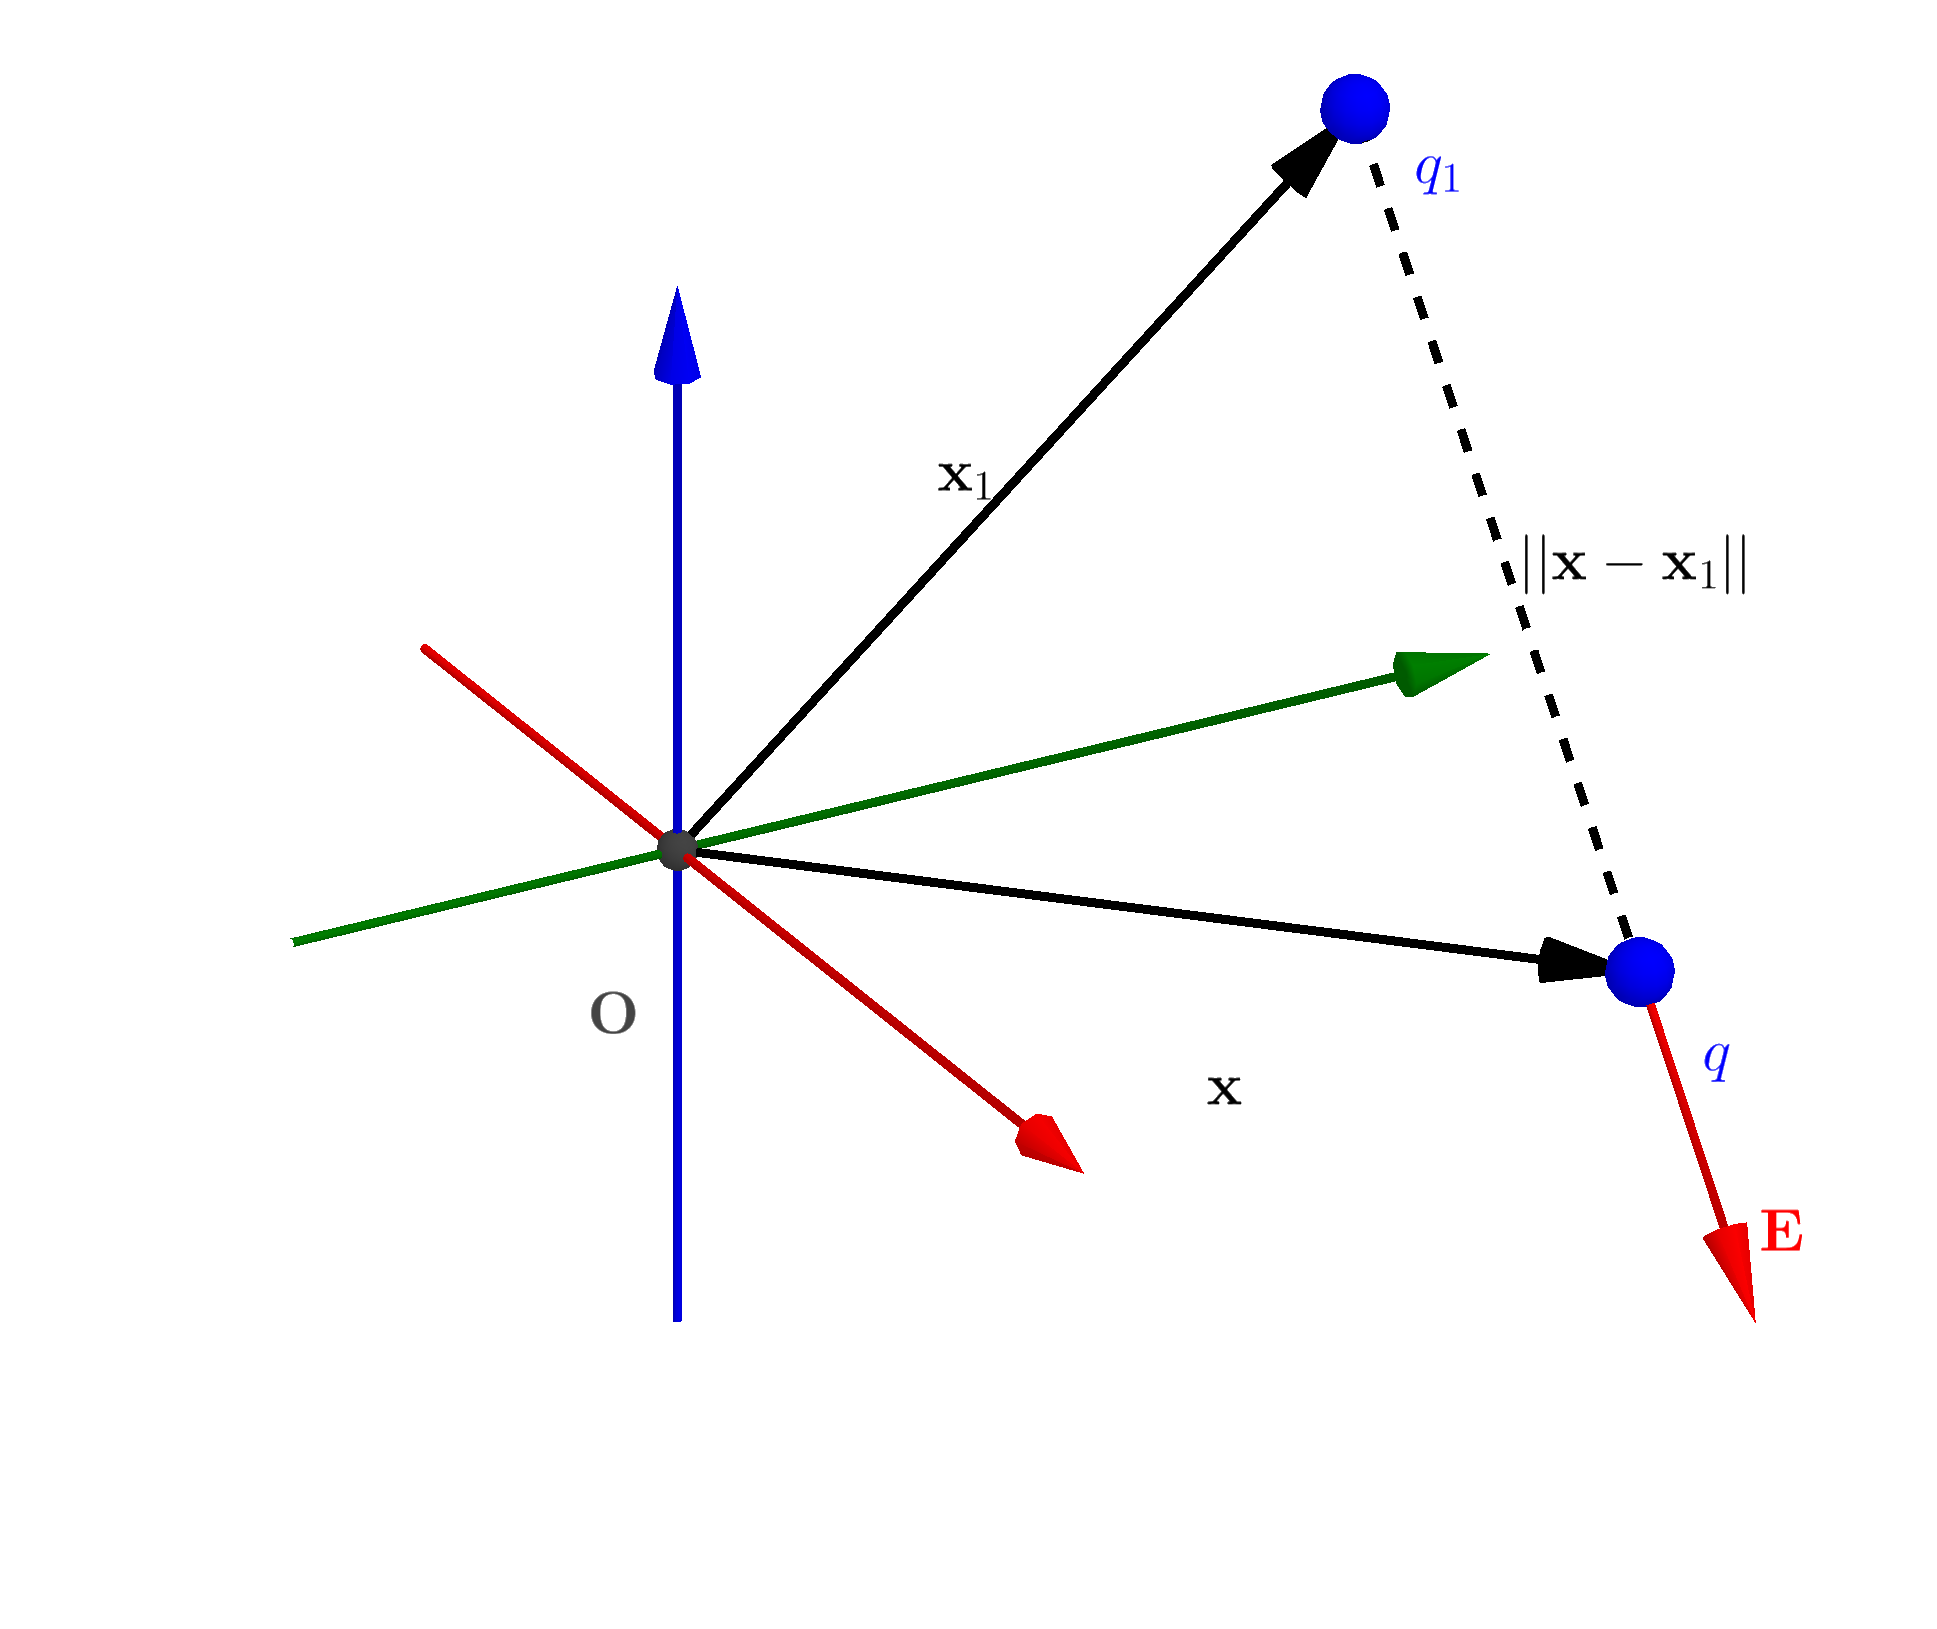
\includegraphics[scale=1]{camp_elet_3D2}}
\caption{}
\label{fig.mossul}
\end{figure}


\section{Equações de Maxwell}

\section{Generalizações da teoria}

\section{Conclusões}